\documentclass[10pt,a4paper]{article}
\usepackage[utf8]{inputenc} % para poder usar tildes en archivos UTF-8
\usepackage[spanish]{babel} % para que comandos como \today den el resultado en castellano
\usepackage{a4wide} % márgenes un poco más anchos que lo usual
\usepackage[conEntregas]{caratula}

\begin{document}
\titulo{Trabajo Práctico Nº1}
\subtitulo{}

\fecha{\today}

\materia{Algoritmos y Estructuras de Datos III}
\grupo{Grupo:}

\integrante{Labate, Martín}{181/15}{martinlabate@gmail.com}
\integrante{Pesaresi, Natalia}{636/14}{natalia.pesaresi@gmail.com}
\integrante{Tilve Neyra, Dana Marlene}{614/14}{tilve.dana@gmail.com}
\integrante{Taboh, Sebastián}{185/13}{sebi\_282@hotmail.com}
% Pongan cuantos integrantes quieran

\maketitle

\documentclass[10pt,a4paper]{article}
\usepackage[utf8]{inputenc} % para poder usar tildes en archivos UTF-8
\usepackage[spanish]{babel} % para que comandos como \today den el resultado en castellano
\usepackage{a4wide} % márgenes un poco más anchos que lo usual

\begin{document}



\definecolor{dkgreen}{rgb}{0,0.6,0}
\definecolor{gray}{rgb}{0.5,0.5,0.5}
\definecolor{mauve}{rgb}{0.58,0,0.82}
\lstset{frame=tb,
  language=Java,
  aboveskip=3mm,
  belowskip=3mm,
  showstringspaces=false,
  columns=flexible,
  basicstyle={\small\ttfamily},
  numbers=none,
  numberstyle=\tiny\color{gray},
  keywordstyle=\color{blue},
  commentstyle=\color{dkgreen},
  stringstyle=\color{mauve},
  breaklines=true,
  breakatwhitespace=true,
  tabsize=3
}


\section{Kaio Ken}

\subsection{Descripción del problema}
\par{El problema se trata de analizar la cantidad de peleas que debe haber entre un grupo de
guerreros, si en cada pelea hay dos bandos a los que pueden pertenecer, para que todos
peleen con todos y en cada pelea estén en uno de los dos bandos. Matemáticamente lo que
proponemos para resolver en problema es: un conjunto, que se divide en dos una cantidad
finita de veces tal que todos los elementos hallan estado en el conjunto opuesto a todos
los demás elementos en elgun momento.}
\par{Observamos que la cantidad de peleas es logarítmica respecto a la cantidad de guerreros o elementos del conjunto principal: si n es potencia de 2 la cantidad de peleas es $\log(n)$ y si n no es potencia de 2 es $\ceil*{\log_2 n}$. Esto es porque en la primer pelea, si establecemos que $\frac{n}{2}$ elementos pertenecen al bando 1 y $\frac{n}{2}$ elementos pertenecen al bando 2, ya tenemos que cada elemento peleó con la mitad del conjunto original. Podemos observar que resta que cada elemento pelee contra sus compañeros de equipo actual. Por lo que, repetimos el paso anterior para cada conjunto de $\frac{n}{2}$ elementos. Y así en $\log_2 n$ peleas cada guerrero habrá peleado con todos los demás, porque el conjunto de n elementos se “divide” en dos cada vez; decimos “divide” porque los equipos son dos siempre: bando 1 y bando 2, pero uso la expresión para explicar cómo obtenemos el resultado de que todos peleen con todos.}
\par{Debemos notar que si la cantidad de elementos es potencia de 2, la cantidad de peleas es exactamente $\log_2 n$. Pero si n no es potencia de 2, voy a necesitar una pelea más para que todos los elementos completen las peleas, es decir que todos terminen de pelear. Esto sucede porque la cantidad de elementos se encuentra entre dos
potencias de 2 (entre $2^{\floor*{\log_2 n}}$ y $2^{\ceil*{\log_2 n}}$), es decir que con ${\floor*{\log_2 n}}$ no alcanza y ${\ceil*{\log_2 n}}$ es el menor número que seguro logra que todos peleen contra todos.}


\subsection{Pseudocódigo}

\begin{algorithm}
\caption{distribuirGuerreros}
\begin{algorithmic}
  \Function{DistribuirGuerreros}{filas: int, columnas: int, matriz: $Arreglo<Arreglo<int>>$ }
	\State int $i \gets 0$ \Comment $\mathcal{O}(1)$
	\State int j \Comment $\mathcal{O}(1)$
	\State int $cambio \gets 0$ \Comment $\mathcal{O}(1)$
	\State int $equipo \gets 1$ \Comment $\mathcal{O}(1)$
	\State int $x \gets 0$ \Comment $\mathcal{O}(1)$
	\While{$i < filas$} \Comment $\mathcal{O}(filas)$
		\State $cambio \gets pow(2,i)$ \Comment $\mathcal{O}(1)$
		\State $x \gets 0$ \Comment $\mathcal{O}(1)$
		\State $j \gets 0$ \Comment $\mathcal{O}(1)$
		\While{$j < columnas$} \Comment $\mathcal{O}(columnas)$
			\If{$x < cambio$} \Comment $\mathcal{O}(1)$
				\State $matriz[i][j] \gets equipo$ \Comment $\mathcal{O}(1)$
			\Else
				\State $equipo \gets ((equipo +1) mod 2)$ \Comment $\mathcal{O}(1)$
				\State $matriz[i][j] \gets equipo$ \Comment $\mathcal{O}(1)$
				\State $x \gets 0$ \Comment $\mathcal{O}(1)$
			\EndIf
			\State $j++$ \Comment $\mathcal{O}(1)$
			\State $x++$ \Comment $\mathcal{O}(1)$
		\EndWhile
		\State $i++$ \Comment $\mathcal{O}(1)$
	\EndWhile
\EndFunction
\end{algorithmic}
\underline{Complejidad:} $\mathcal{O}(filas*columnas)$\\
\end{algorithm}


\begin{algorithm}
\caption{KaioKen}
\begin{algorithmic}
  \Function{Kaioken}{n: int}
	\State int $filas \gets \ceil*{\log_2 n}$ \Comment $\mathcal{O}(1)$
	\State int m[filas][n] \Comment $\mathcal{O}(1)$
	\State distribuirGuerreros(filas, n, m) \Comment $\mathcal{O}(filas*n) = \mathcal{O}(\ceil*{\log_2 n}*n)$
	\\
	\State int $i \gets 0$ \Comment $\mathcal{O}(1)$
	\State int j \Comment $\mathcal{O}(1)$
	\\
	\State imprimir ~filas \Comment $\mathcal{O}(1)$
	\While{$i < filas$} \Comment $\mathcal{O}(filas) = \mathcal{O}(\ceil*{\log_2 n})$
		\State $j \gets 0$ \Comment $\mathcal{O}(1)$
		\While{$j < n$} \Comment $\mathcal{O}(n)$
			\State imprimir ~$m[i][j]+1$ \Comment $\mathcal{O}(1)$
			\State $j++$ \Comment $\mathcal{O}(1)$
			\If{$j < n$} \Comment $\mathcal{O}(1)$
				\State imprimir ~"~ " \Comment $\mathcal{O}(1)$
			\EndIf
		\EndWhile
		\State $i++$ \Comment $\mathcal{O}(1)$
	\EndWhile
\EndFunction
\end{algorithmic}
\underline{Complejidad:} $\mathcal{O}(\log _{2} n * n)$\\
    \underline{Justificación:} $ \mathcal{O}(\ceil*{\log_2 n}*n)$ + $ \ceil*{\log_2 n} * \mathcal{O}(n)$ = $2*\mathcal{O}(\log _{2} n * n)$ = $\mathcal{O}(\log _{2} n * n)$\\
\end{algorithm}

\newpage
\subsection{Demostración de optimalidad}
Se parte de un grupo de $n$ guerreros y se divide en dos grupos de $n/2$ (si n es par; si no, se divide en un grupo de $\ceil*{n/2}$ y en otro de $\floor*{n/2}$). A su vez, cada uno de estos se partirá a la mitad.
Esto se debe a que para pelear a los n guerreros todos con todos se puede organizar una pelea de $n/2$ contra $n/2$ y luego pelear a cada uno de esos conjuntos todos con todos.
\par{Así, se consigue un árbol exactamente binario porque siempre los grupos se dividen en 2 equipos. Las divisiones en equipos terminan cuando quedan $n$ grupos de 1 guerrero porque en ese caso ya habrán peleado todos con todos los $n$ guerreros, es decir, cuando queda un árbol binario con $n$ hojas. Por otro lado, la altura de este árbol es la cantidad de peleas globales que se necesitó organizar, y sabemos que la altura del árbol es mínima cuando el árbol es balanceado, que de hecho es una propiedad que cumple el árbol resultante de dividir siempre a la mitad. Así, se concluye que esta forma de división resulta en el óptimo de peleas globales, que es igual a $\ceil*{\log_2 n}$.}
\par{Esta es la misma explicación de por qué en mergeSort se divide el arreglo a la mitad.}

\subsection{Cota de complejidad}
\par{Como está detallado en el Algoritmo 3, la complejidad del algoritmo propuesto para KaioKen resulta $\mathcal{O}(\log _{2} n * n)$ y de hecho también es $\mathcal{\theta}(\log _{2} n * n)$}.
\par{Este algoritmo no tiene ni mejor ni peor caso dado que siempre se realiza la misma cantidad de operaciones en función de n. Cabe resaltar que en este problema para un determinado tamaño de entrada no se pueden tener diferentes situaciones y el programa siempre lleva a cabo cada instrucción una cantidad fija de veces que depende del n.}
\par{Como se verá más adelante, esto no es así en el Problema 2, en el que puede haber un mismo tamaño de entrada con situaciones muy distintas y disposiciones de androides totalmente diferentes, dando lugar a un mejor y un peor caso del algoritmo propuesto para resolver ese problema. Como en ese caso la información puede ser distinta para un mismo tamaño de entrada cada instrucción se correrá una cantidad de veces que depende de esa información, dando lugar a mayores y menores tiempos de ejecución para el mismo tamaño de entrada.}

\newpage
\subsection{Experimentación}
Realizamos la medición del tiempo de ejecución de la parte del código que calcula la solución y recolectamos los datos expuestos en la siguiente tabla:

\begin{table}[h!]
\centering
\label{my-label}
\begin{tabular}{cc}
\hline
\multicolumn{1}{|c|}{n (Tamaño de la entrada)} & \multicolumn{1}{c|}{Tiempo promedio (nanosegundos)}                                                                                                                                    \\ \hline
\multicolumn{1}{|c|}{10000}                        & \multicolumn{1}{c|}{1689}                                                                                                                                     \\ \hline
\multicolumn{1}{|c|}{15000}                        & \multicolumn{1}{c|}{1889}                                                                                                                                     \\ \hline
\multicolumn{1}{|c|}{20000}                        & \multicolumn{1}{c|}{3051}                                                                                                                                     \\ \hline
\multicolumn{1}{|c|}{25000}                        & \multicolumn{1}{c|}{3616}                                                                                                                                     \\ \hline
\multicolumn{1}{|c|}{30000}                        & \multicolumn{1}{c|}{3794}                                                                                                                                     \\ \hline
\multicolumn{1}{|c|}{35000}                        & \multicolumn{1}{c|}{5612}                                                                                                                                     \\ \hline
\multicolumn{1}{|c|}{40000}                        & \multicolumn{1}{c|}{5735}                                                                                                                                     \\ \hline
\multicolumn{1}{|c|}{45000}                        & \multicolumn{1}{c|}{6550}                                                                                                                                     \\ \hline
\multicolumn{1}{|c|}{50000}                        & \multicolumn{1}{c|}{5798}                                                                                                                                     \\ \hline
\multicolumn{1}{|c|}{55000}                        & \multicolumn{1}{c|}{9041}                                                                                                                                     \\ \hline
\multicolumn{1}{|c|}{60000}                        & \multicolumn{1}{c|}{8217}                                                                                                                                     \\ \hline
\multicolumn{1}{|c|}{65000}                        & \multicolumn{1}{c|}{9236}                                                                                                                                     \\ \hline
\multicolumn{1}{|c|}{70000}                        & \multicolumn{1}{c|}{8781}                                                                                                                                     \\ \hline
\multicolumn{1}{|c|}{75000}                        & \multicolumn{1}{c|}{8025}                                                                                                                                     \\ \hline
\multicolumn{1}{|c|}{80000}                        & \multicolumn{1}{c|}{8841}                                                                                                                                     \\ \hline
\multicolumn{1}{|c|}{85000}                        & \multicolumn{1}{c|}{12973}                                                                                                                                     \\ \hline
\multicolumn{1}{|c|}{90000}                        & \multicolumn{1}{c|}{16051}                                                                                                                                     \\ \hline
\multicolumn{1}{|c|}{95000}                        & \multicolumn{1}{c|}{17312}                                                                                                                                     \\ \hline
\multicolumn{1}{|c|}{100000}                        & \multicolumn{1}{c|}{18256}                                                                                                                                     \\ \hline

\end{tabular}
\caption{Tabla que muestra los tiempos de ejecución correspondientes a distintos tamaños de entrada.}
\end{table}

\par{El gráfico asociado a este experimento es:}
\begin{figure}[h!]
  \centering
  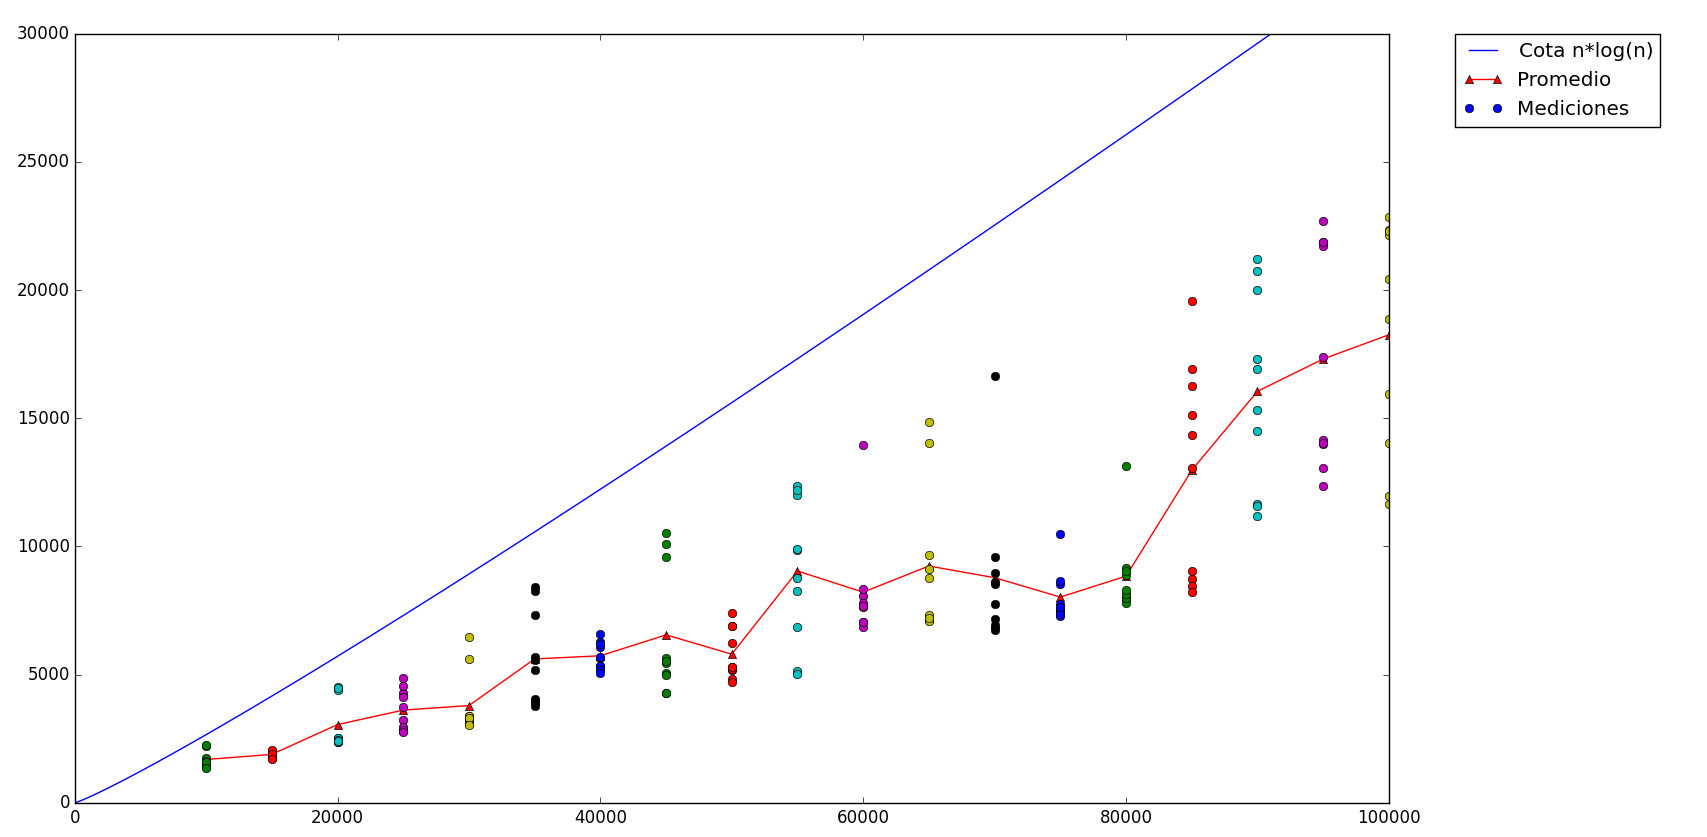
\includegraphics[width=12cm, height=9cm]{tiemposEj1Nuevos}
  \caption{Tiempos de ejecución para distintas entradas. La curva azul es la curva de la complejidad, $n \times \log n$, multiplicada por 0.02, y la roja caso aleatorio.}
\end{figure}

\newpage

\subsection{Apéndice: código de KaioKen}
\begin{lstlisting}
#include <math.h>
#include <stdlib.h>
#include <iostream>
using namespace std;

void kaioKen(int);

int main(int argc, char* argv[]){
	int i;
	cin >> i;
	kaioKen(i);
	return 0;
}

void kaioKen(int n){
	int filas = ceil(log2(n));
	int equipo = 1;
	int cambio = 0;
	int x = 0;
	int m [filas][n];

	//Distribuimos los guerreros
	for (int i = 0; i < filas; i++){
		cambio = pow(2,i);
		x = 0;
		for(int j = 0; j < n; j++){
			if(x < cambio){
				m[i][j] = equipo;
			}else{
				equipo = ((equipo +1) % 2);
				m[i][j] = equipo;
				x = 0;
			}
			x++;
		}
	}

	cout << filas << endl;
	for(int i = 0; i < filas; i++){
		for(int j = 0; j < n; j++){
			cout << m[i][j]+1;
			if (j < n) {
				std::cout << " ";
			}
		}
		cout << endl;
	}
}
\end{lstlisting}

\documentclass[10pt,a4paper]{article}
\usepackage[utf8]{inputenc} % para poder usar tildes en archivos UTF-8
\usepackage[spanish]{babel} % para que comandos como \today den el resultado en castellano
\usepackage{a4wide} % márgenes un poco más anchos que lo usual
\usepackage{listings}
\usepackage{color}

\begin{document}

\definecolor{dkgreen}{rgb}{0,0.6,0}
\definecolor{gray}{rgb}{0.5,0.5,0.5}
\definecolor{mauve}{rgb}{0.58,0,0.82}
\lstset{frame=tb,
  language=Java,
  aboveskip=3mm,
  belowskip=3mm,
  showstringspaces=false,
  columns=flexible,
  basicstyle={\small\ttfamily},
  numbers=none,
  numberstyle=\tiny\color{gray},
  keywordstyle=\color{blue},
  commentstyle=\color{dkgreen},
  stringstyle=\color{mauve},
  breaklines=true,
  breakatwhitespace=true,
  tabsize=3
}

\section{Genkidama}

\subsection{Descripcion del problema}
\begin{verbatim}
El problema a resolver es el siguiente:
Tenemos un secuencia de puntos (x,y) en el espacio para los cuales, si la coordenada x de un punto es mayor a la de otro punto, la coordenada en y del segundo punto es menor. Dado un valor T, se desea calcular la minima cantidad de gendikamas a tirar para destruir a todos los puntos. Si se tira a un punto (x0,y0), al gendikama alcanza a destruir a todos los puntos que posean x<=x0+t y posean y<=y0+t.

Para resolverel problema:
Definamos el área de impacto $ A: \mathbb{{N_{0}}^2 ~x~ N} \rightarrow \mathbb{Z^2}$ como $A(P,T) = \{ (x, y) \in \mathbb{Z^2} : 0 \leq x \leq P_{x}+T ~ \wedge 0 \leq y \leq P_{y}+T \}$, es decir, el conjunto de puntos del plano en los que en caso de haber androides estos morirían por la Gendikama tirada en P. Con esta idea de área de impacto se puede pensar que no aporta tener en cuenta el área por sobre el objetivo vivo de mayor coordenada en $y.$
Va a haber que eliminar al objetivo situado en $A$. Se puede tirar una Gendikama al punto A, pero surge la pregunta de si se podría hacer algo mejor. ¿Qué pasa si se dispara a $B$? Si $ A_{y} \leq B_{y}+T$ entonces el área de impacto $A(B,T)$ incluye al punto $A$. Así, sería mejor disparar la Gendikama a $B$ que a $A$ dado que como $ A_{x} < B_{x}$ entonces $ A_{x}+T < B_{x}+T$, lo que nos da una idea intuitiva de inclusión de áreas, $A(A,T) \subset A(B,T)$ (nótese que la inclusión es estricta) y podemos decir que diparar a B es más destructivo.
Así, volvemos a preguntarnos: ¿Qué pasa si se dispara a C? ¿Esto también mataría a A?
Si sí, seguimos preguntándonos por el siguiente punto de menor coordenada $y$, y podemos tener dos situaciones:

- Recorrer hasta el último punto y que una Gendikama lanzada ahí también elimine al androide situado en A, necesitando sólo un disparo para destruir a todos.
- Recorrer hasta eventualmente encontrar un androide posicionado en un punto $K$ al que si se lanzara una Gendikama ésta no matara al androide en A. En este caso habría que disparar al androide situado en la posición con la coordenada $y$ inmediatamente anterior a la de $K$, llamémoslo J, y calcular $J_{x}+T$ para ver cuál sería el objetivo de mayor coordenada $y$ que quedara vivo  y repetir el proceso como si este fuera el nuevo $A$. Si no quedara ningún objetivo por eliminar entonces ya no habría necesidad de seguir disparando Gendikamas.

Ejemplos útiles

Supongamos que tenemos los puntos mostrados en [Ejemplo Inicial Útil] y $T = 1$.
Primero queremos destruir al objetivo situado en $A$. Miramos el objetivo $B$, que tiene la mayor coordenada $y$ de los que tienen menor coordenada $y$ que $A$ (que son todos dado que se empieza queriendo destruir al objetivo situado en el punto con mayor $y$). En la Figura .. [T=1: Ejemplo área 1] vemos que $A_{y} > B_{y} + T$ y que A no pertenece al área de impacto A(B, 1), o sea que disparar una genkidama al punto B no eliminaría al androide de A. Por transitividad, como $B_{y} > C_{y} > ... > F_{y}$, ninguno de los disparos a los puntos siguientes a B eliminará al objetivo de A, por lo que es necesario disparar una genkidama a A. El área de impacto A(A, T) = A( (1,8), 1) de esta genkidama, sombrada con rojo en la Figura .. [T=1: Ejemplo área 1], incluye al punto B, que además es el de mayor coordenada $x$ de los destruidos por esta gendikama. 
El siguiente a B, C, es el de mayor coordenada $y$ de los que están vivos, y se repite el proceso que se llevó a cabo con A. En [T=1: Ejemplo área 2] se ve que la segunda gendikama se disparará a D, destruyendo a los objetivos de C, D y E.
Finalmente queda la situación mostrada en [T=1: Ejemplo área 3] y se dispara una tercera genkidama a F.

Ahora veamos cómo sería este proceso con $T = 2$.
De vuelta se comienza queriendo destruir al objetivo en A. Como se ve en la Figura .. [T = 2: Ejemplo área 1], disparar a C no destruye a A pero disparar a B sí. Así, morirán los androides situados en los puntos incluidos en la región sombreada naranja en la Figura .. [T = 2: Ejemplo área 2] (el área de impacto A(B, 2)).
Finalmente queda la situación mostrada en [T = 2: Ejemplo área 3] en la que el objetivo es destruir al objetivo de E y se terminará disparando a F eliminando a los dos androides restantes.
En este caso se habrá destruido a todos los androides utilizando dos genkidamas.
\end{verbatim}

\subsection{Pseudocódigo}
\begin{verbatim}
\end{verbatim}

\subsection{Cota de complejidad}
\begin{verbatim}
\end{verbatim}

\subsection{Extracto importante de código}
%%no esta actualizado
\begin{lstlisting}
void genkidama(int, int, vector<tuple<int, int>>);
int indiceDeMenorYQueLoMata(int, int, vector<tuple<int,int>>);
int indiceDeMayorXQueMata(int, int, vector<tuple<int,int>>);
void destruir();

int main(){
	int t;
	int n;
	cin >> n >> t;
	vector<tuple<int,int>> e;
	tuple<int,int> en;
	int x;
	int y;
	for (int i = 0; i < n; i++) {
		cin >> x >> y;
		en = make_tuple(x,y);
		e.push_back((en));
	}
	genkidama(t, n, e);
	return 0;
}

// Toma el t, el indice del objetivo en e y el vector de tuplas.
int indiceDeMenorYQueLoMata(int t, int indiceDeObjetivo, vector<tuple<int,int>> e){
	int j = indiceDeObjetivo - 1;
	while((j >= 0) && ((get<1>(e[j]) + t) >= get<1>(e[indiceDeObjetivo]))){
		j--;
	}
	j++;
	return j;
}

int indiceDeMayorXQueMata(int t, int indiceDeObjetivo, vector<tuple<int,int>> e){
	int distanciaDeDano = get<0>(e[indiceDeObjetivo]) + t;
	int i = indiceDeObjetivo - 1;
	while((i >= 0) && (get<0>(e[i]) <= distanciaDeDano)){
		i--;
	}
	i++;
	return i;
}

void destruir(int t, int indiceDeObjetivo, vector<tuple<int,int>> e, int genkidamas, int indicePorArea){
	indicePorArea = indiceDeMayorXQueMata(t, indiceDeObjetivo, e) - 1;
	genkidamas++;
}


// MODULARIZADO
void genkidama(int t, int n, vector<tuple<int,int>> e){
	assert (n > 0 && n == e.size() && "La cantidad de enemigos es distinta a la cantidad de posisciones");
	vector<int> atacados;
	int genkidamasUtilizadas = 0;
	int indiceDeObjetivoPorArea = n-1;
	// el de arriba es aquel al que quiero que le llegue la onda expansiva
	bool hayAlgunoVivo = true;
	while(hayAlgunoVivo){
		// el de abajo es aquel al que le voy a tirar la bomba
		int indiceDeObjetivo = indiceDeMenorYQueLoMata(t, indiceDeObjetivoPorArea, e);
		atacados.push_back(indiceDeObjetivo + 1);
		// el +1 de arriba surge de que en el enunciado se enumeran desde el 1 y
		// nosotros enumeramos desde 0
		hayAlgunoVivo = !(indiceDeMayorXQueMata(t, indiceDeObjetivo, e) == 0);
		destruir(t, indiceDeObjetivo, e, genkidamasUtilizadas, indiceDeObjetivoPorArea);
	}
		std::cout << genkidamasUtilizadas << std::endl;
		int h = 0;
		while (h < genkidamasUtilizadas) {
				std::cout << atacados[h];
				h++;
				if (h < genkidamasUtilizadas) {
						std::cout << " ";
				}
		}
}
\end{lstlisting}

\subsection{Experimentacion}
\begin{verbatim}
\end{verbatim}

\end{document}

\documentclass[10pt,a4paper]{article}
\usepackage[utf8]{inputenc} % para poder usar tildes en archivos UTF-8
\usepackage[spanish]{babel} % para que comandos como \today den el resultado en castellano
\usepackage[margin=2cm]{geometry}
\usepackage{amsmath}
\usepackage{listings}
\usepackage{color}
\usepackage{graphicx}
\usepackage{wrapfig}
\usepackage{algorithm}
\usepackage{algpseudocode}
\usepackage{mathtools}

\begin{document}

\definecolor{dkgreen}{rgb}{0,0.6,0}
\definecolor{gray}{rgb}{0.5,0.5,0.5}
\definecolor{mauve}{rgb}{0.58,0,0.82}
\lstset{frame=tb,
  language=Java,
  aboveskip=3mm,
  belowskip=3mm,
  showstringspaces=false,
  columns=flexible,
  basicstyle={\small\ttfamily},
  numbers=none,
  numberstyle=\tiny\color{gray},
  keywordstyle=\color{blue},
  commentstyle=\color{dkgreen},
  stringstyle=\color{mauve},
  breaklines=true,
  breakatwhitespace=true,
  tabsize=3
}

\section{Kamehameha}

\subsection{Descripcion del problema}

El problema consiste en calcular la mínima cantidad de Kamehamehas que debe lanzar Goku para destruir un cunjunto de andriodes usando Backtracking.
Al usar backtracking, el problema se reduce a trazar todas las posibles rectas que pasan una sola vez por cada punto y elegir la combinación con menor cantidad de rectas. Por ejemplo, si hay 5 androides en las siguientes posiciones
1 (1,2) 2 (2,1) 3 (3,2) 4 (4,2) 5 (3,3)
Como muestra el siguiente gráfico
\begin{figure}[h!]
  \centering
  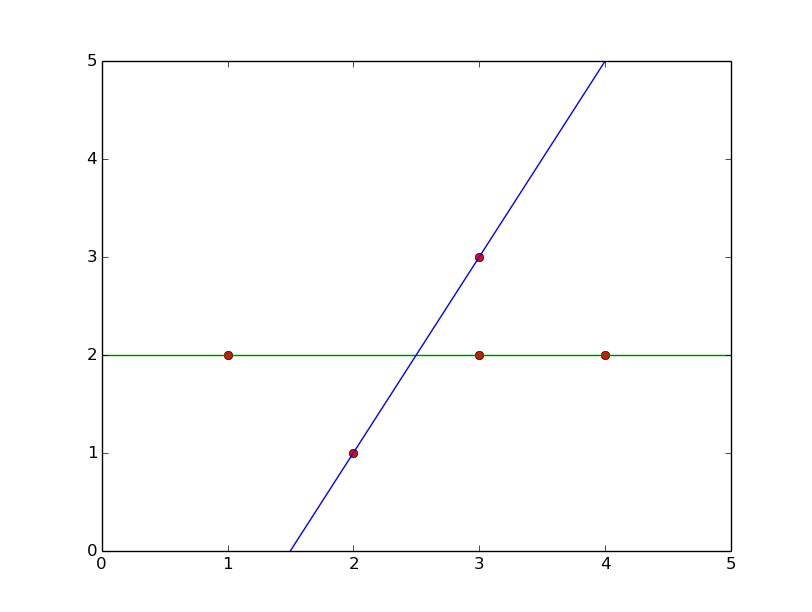
\includegraphics[width=7cm, height=6cm]{ejemploHame1}
  \caption{Puntos distribuidos inicialmente.}
\end{figure}

Una posible solución óptima sería lanzar 2 Kamehameha, 1 que mate a 3 androides (al 1, 3 y 4), la recta verde, y otro que mate a los otros 2, la recta azul.

\subsection{Descripción de la resolución}
La idea del algoritmo es que recursivamente vaya creando todas las combinaciones de rectas. Esto lo logramos utilizando una función principal, Kamehameha, a la que recurrimos y 2 funciones, una que se fija si un androide puede ser atacado con un Kamehameha ya lanzado (si esta alineado con algun con algun otro grupo de androides ya atacados) y vuelve a llamar a la función principal con los nuevos valores una vez por cada grupo con el que esta alineado este androide y otra función que comienza un nuevo ataque con ese androide y vuelve a llamar a la función principal. De esta forma, probando con un enemigo, volviendo atras, probando con el siguiente, volviendo atras y asi sucesivamente hasta probar con todos los enemigos, podemos generar todas las posibles combinaciones de líneas. Lo único que resta es verificar cual de estas es la óptima. Para conseguirlo, cada vez que generamos una solución completa, verificamos su tamaño (su acantidad de líneas) y la guardamos si es la menor hasta el momento, sino la descartamos.
Para mejorar el tiempo de ejecución decidimos agregar un a poda que descarta soluciones que estan siendo generadas en el momento que su tamaño supera el tamaño de la solución minima alamacenada, ya que sabemos que si o si es mayor o igual a la que ya tenemos, por lo tanto no nos sirve.

\subsection{Pseudocódigo}
\begin{verbatim}
\end{verbatim}

\subsection{Cota de complejidad}
\paragraph{Como ya explicamos, usamos recursividad y 2 funciones. En cada llamado recursivo usamos las 2 funciones. La que genera un nuevo ataque es O(1) ya que hace una cantidad acotada de operaciones O(1). La otra, verifica si un enemigo esta alineado con los otros una vez por cada ataque realizado hasta el momento. Lala cantidad de ataques es acotada, ya que como cualqueir par de puntos puede ser unido con una recta, la cantidad de ataques o rectas necesarios es menor o igual a $n/2$, siendo $n$ la cantidad total de enemigos. De esta forma vemos que esta función es O($n/2$).

}

\subsection{Extracto importante de código}
\begin{lstlisting}
typedef pair<int,int> posicion_t;
typedef vector<posicion_t> Kamehameha_t;
typedef vector<Kamehameha_t> Kamehamehas_t;
typedef deque<posicion_t> listaPos_t;

int minimo_global = std::numeric_limits<int>::max();
listaPos_t enemigos_global;
Kamehamehas_t mejor_configuracion;

void Kamehameha(listaPos_t enemigos,
                Kamehamehas_t enLaMira,
                int indexRectaActual);
void atacarEnAtaqueActual(posicion_t enemigo,
                          listaPos_t restoEnemigos,
                          Kamehamehas_t ataques,
                          int nroAtaque);
void atacarEnNuevoAtaque(posicion_t enemigo,
                         listaPos_t restoEnemigos,
                         Kamehamehas_t ataques,
                         int nroAtaque);
bool alineados (Kamehameha_t atacados, posicion_t enemigo);
void reporte(listaPos_t enemigos, Kamehamehas_t ataques, int nroAtaque);
int buscarPosicion(const posicion_t& enemigo);
void mostrarSolucion();

int main() {
    int cantEnemigos;
    cin >> cantEnemigos;
    listaPos_t enemigos;
    Kamehamehas_t enLaMira;
    Kamehameha_t kamehameha;
    enLaMira.push_back(kamehameha);
    int indexRectaActual;
	posicion_t posicion;
    srand(time(NULL));
    for (int i = 0; i < cantEnemigos; i++) {
        int x = rand() %10;
        int y = rand() %10;
    	posicion = make_pair(x, y);
    	enemigos.push_back((posicion));
    }
    //Para imprimir las tuplas generadas al azar:
    enemigos_global = enemigos;
    for (listaPos_t::iterator it = enemigos.begin(); it != enemigos.end(); ++it) {
            cout << (*it).first << " " << (*it).second << endl;
    }
    Kamehameha(enemigos, enLaMira, 0);
    mostrarSolucion();
    return 0;
}

void Kamehameha(listaPos_t enemigos, Kamehamehas_t ataques, int nroAtaque) {
    if (enemigos.size() == 0) {
        if (minimo_global > (int)ataques.size()) {
            minimo_global = (int) ataques.size();
            mejor_configuracion = ataques;
        }
    } else {
        for (int i = 0; i < enemigos.size(); i++) {
            posicion_t enemigo = enemigos.front();
            enemigos.pop_front();
            atacarEnAtaqueActual(enemigo, enemigos, ataques, nroAtaque);
            atacarEnNuevoAtaque(enemigo, enemigos, ataques, nroAtaque);
            enemigos.push_front(enemigo);
        }
    }
}

void atacarEnAtaqueActual(posicion_t enemigo, listaPos_t restoEnemigos, Kamehamehas_t ataques, int nroAtaque) {
    Kamehameha_t atacados = ataques[nroAtaque];
    if (atacados.size() == 0){
        Kamehameha_t comenzarAtaque;
        comenzarAtaque.push_back(enemigo);
        ataques[nroAtaque] = comenzarAtaque;
        Kamehameha(restoEnemigos, ataques, nroAtaque);
        Kamehameha_t reestablecerAtaque;
        ataques[nroAtaque] = reestablecerAtaque;
    } else if (alineados(atacados, enemigo)) {
        ataques[nroAtaque].push_back(enemigo);
        Kamehameha(restoEnemigos, ataques, nroAtaque);
        ataques[nroAtaque].pop_back();
    } else {
        return;
    }
}

void atacarEnNuevoAtaque(posicion_t enemigo, listaPos_t restoEnemigos, Kamehamehas_t ataques, int nroAtaque) {
    if (ataques[nroAtaque].size() > 0) {
        Kamehameha_t comenzarAtaque;
        comenzarAtaque.push_back(enemigo);
        ataques.push_back(comenzarAtaque);
        nroAtaque++;
        Kamehameha(restoEnemigos, ataques, nroAtaque);
        nroAtaque--;
        ataques.pop_back();
    }
}

bool alineados (Kamehameha_t atacados, posicion_t enemigo) {
    if (atacados.size() == 0 || atacados.size() == 1) {
        return true;
    } else {
        posicion_t primero = atacados[0];
        posicion_t segundo = atacados[1];
        int termino1 = segundo.second - primero.second;
        int termino2 = enemigo.first - primero.first;
        int termino3 = enemigo.second - primero.second;
        int termino4 = segundo.first - primero.first;
        return termino1*termino2 == termino3*termino4;
    }
}

void reporte(listaPos_t enemigos, Kamehamehas_t ataques, int nroAtaque) {
    cout << "enemigos: ";
    for (listaPos_t::iterator itL = enemigos.begin(); itL != enemigos.end(); ++itL) {
        cout << "(" << (*itL).first << ", " << (*itL).second << ")";
        if (itL!= enemigos.end()) {
            cout << ", ";
        }
    }
    cout << endl ;
    for (int i = 0; i < ataques.size(); i++) {
        Kamehameha_t ataqueEnIdx = ataques[i];
        cout << "[";
        for (Kamehameha_t::iterator it = ataqueEnIdx.begin(); it != ataqueEnIdx.end(); ++it) {
            cout << "(" << (*it).first << ", " << (*it).second << "), ";
            if (it!= ataqueEnIdx.end()){ cout << ", "; };
        }
        cout << "]" << endl;
    }
}

void mostrarSolucion() {
    cout << mejor_configuracion.size() << endl;
    for (int i = 0; i < mejor_configuracion.size(); i++) {
        Kamehameha_t ataqueEnIdx = mejor_configuracion[i];
        cout << ataqueEnIdx.size() << " ";
        for (Kamehameha_t::iterator it = ataqueEnIdx.begin(); it != ataqueEnIdx.end(); ++it) {
            cout << (buscarPosicion(*it)+1) << " ";
        }
        cout << endl;
    }
}

int buscarPosicion(const posicion_t& enemigo) {
    listaPos_t::iterator it = find (enemigos_global.begin(), enemigos_global.end(), enemigo);
    return distance(enemigos_global.begin(), it);
}
\end{lstlisting}

\subsection{Experimentacion}
\begin{verbatim}
Se puede observar que el tiempo que tarda el algoritmo es relativo a la distribucion de los puntos, aunque principalmente a la cantidad que sean. A partir de 16 puntos el algoritmo tarda mas de un minuto.

Cantidad de puntos = 1
Posiciones = 9 8
El tiempo que tardo es:1.7e-05
Rectas que necesitamos = 1
1 1 

Cantidad de puntos = 2
Posiciones = 12 5 - 9 3
El tiempo que tardo es:3.2e-05
Rectas que necesitamos = 1
2 1 2 
   
Cantidad de puntos = 3
Posiciones = 6 3 - 14 7 - 3 12
El tiempo que tardo es:4.4e-05
Rectas que necesitamos = 2
2 1 2 
1 3 
   
Cantidad de puntos = 4
Posiciones = 13 0 - 1 12 - 9 10 - 10 1
El tiempo que tardo es:6e-05
Rectas que necesitamos = 2
2 1 2 
2 3 4 
   
Cantidad de puntos = 5
Posiciones = 9 0 - 11 6 - 14 12 - 12 8 - 5 9
El tiempo que tardo es:0.000175
Rectas que necesitamos = 2
2 1 5 
3 2 3 4 
   
Cantidad de puntos = 6
Posiciones = 5 4 - 0 11 - 1 7 - 3 9 - 10 10 - 12 3
El tiempo que tardo es:0.000169
Rectas que necesitamos = 3
2 1 2 
2 3 4 
2 5 6 
   
Cantidad de puntos = 7
Posiciones = 12 9 - 7 13 - 5 10 - 10 14 - 9 7 - 0 3 - 11 8
El tiempo que tardo es:0.000836
Rectas que necesitamos = 4
2 1 2 
2 3 4 
2 5 6 
1 7 
   
Cantidad de puntos = 8
Posiciones = 6 13 - 7 3 - 1 0 - 4 10 - 8 6 - 3 9 - 0 5 - 12 2
El tiempo que tardo es:0.00056
Rectas que necesitamos = 3
3 1 6 7 
2 2 3 
3 4 5 8 
   
Cantidad de puntos = 9
Posiciones = 7 11 - 12 2 - 8 0 - 0 3 - 13 12 - 6 5 - 1 7 - 3 6 - 9 1
El tiempo que tardo es:0.006745
Rectas que necesitamos = 5
2 1 2 
2 3 4 
2 5 6 
2 7 8 
1 9 
   
Cantidad de puntos = 10
Posiciones = 6 9 - 4 12 - 2 14 - 8 7 - 3 3 - 9 10 - 5 4 - 11 6 - 10 13 - 14 2
El tiempo que tardo es:0.002715
Rectas que necesitamos = 4
2 1 5 
3 2 3 10 
3 4 6 9 
2 7 8 
   
Cantidad de puntos = 15
Posiciones = 0 2 - 5 5 - 14 8 - 3 13 - 9 4 - 7 14 - 8 12 - 12 1 - 10 11 - 6 3 - 4 9 - 13 7 - 11 6 - 2 0 - 1 10
El tiempo que tardo es:0.785094
Rectas que necesitamos = 7
2 1 2 
2 3 4 
2 5 6 
2 7 10 
3 8 9 13 
2 11 12 
2 14 15 

Gafico que representa este experimento:

\end{verbatim}

\end{document}


\subtitle{Conclusiones}
\paragraph{Aquí las conclusiones del TP.}

\end{document}

\end{document}
